\apendice{Documentación de usuario}

\section{Introducción}
En este apartado, se detallará un manual sobre como hacer uso del sistema implementado. 

\section{Requisitos de usuarios}
Los requisitos mínimos para poder hacer uso del sistema completo son:

\begin{itemize}
\item Contar con un ordenador con el sistema operativo deseado.
\item Disponer de un navegador Web. Se recomienda el uso de \emph{Google Chrome}, \emph{Mozilla Firefox} o Safari. Se ha probado el entorno en los tres navegadores. \emph{Chromium} ha presentado problemas en el \emph{parseo} del mensaje \emph{SDP}\footnote{Session Description Protocol, detallado en la memoria técnica del proyecto} proveniente del servidor WebRTC que implementa \emph{UV4L}, y no se recomienda. Se desaconseja por completo el uso de \emph{Internet Explorer} o \emph{Edge}. 
\item \emph{Opcional}. Contar con una emisora detectable por el sistema operativo como un \emph{joystick}, para poder hacer uso de las características de control remoto del sistema.
\item Conexión a internet.
\end{itemize}

\section{Instalación}
\label{sec:instTaranis}
El usuario final accederá a la aplicación a través de una interfaz web, así que no se requiere instalar ningún \emph{software} adicional. 

Sí que se detalla a continuación el proceso de conexionado y configuración de la emisora para hacer uso del control remoto. Para el desarrollo del proyecto se ha utilizado una emisora \emph{FrSky Taranis X9D plus}. Dicho modelo es tanto hardware, como código abierto. 

\begin{enumerate}
\item Descargar \href{http://www.open-tx.org/downloads}{OpenTX} y seguir el asistente de instalación. 
\item Abrir OpenTX.
\item Encender la emisora pulsando la siguiente combinación de botones, los dos botones laterales se deben dirigir hacia dentro, y el botón de encender (central) hacia arriba: 
 \begin{figure}[H]
	\centering
	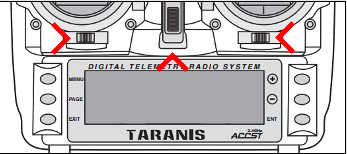
\includegraphics[width=0.7\textwidth]{opentxboot}
	\caption[Emisora en modo bootloader]{Encender emisora en modo \emph{bootloader}.}\label{fig:opentxboot}
\end{figure}
\item Conectar el cable USB a la emisora. El sistema la detectará como un medio de almacenamiento externo, ya que esta emisora dispone de lector de tarjetas microSD para guardar los modelos y configuración de los mismos.

\begin{figure}[H]
	\centering
	\includegraphics[width=0.9\textwidth]{taranisUSB}
	\caption[Emisora conectada]{Conexión de emisora a \emph{OpenTX}}\label{fig:taranisUSB}
\end{figure}

\item Pulsar sobre \emph{Read models and settings from radio} para leer la información de la radio. Tanto los modelos como la configuración.
\begin{figure}[H]
	\centering
	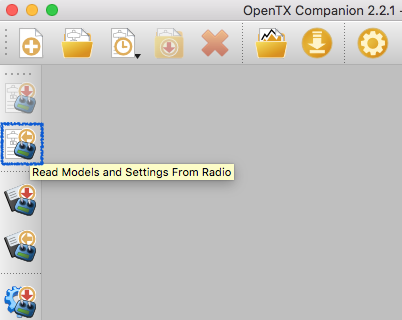
\includegraphics[width=0.7\textwidth]{opentxread}
	\caption[Lectura de modelos OpenTX]{Lectura de modelos mediante \emph{OpenTX}.}\label{fig:opentxread}
\end{figure}

\item En la lista de modelos, añadir uno nuevo pulsando sobre \emph{Add model}.
\begin{figure}[H]
	\centering
	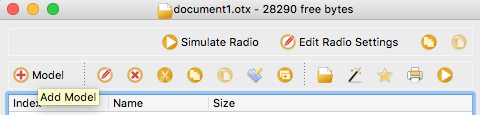
\includegraphics[width=0.7\textwidth]{opentxadd}
	\caption[Creación de modelos OpenTX]{Creación de modelos mediante \emph{OpenTX}.}\label{fig:opentxadd}
\end{figure}

\item A continuación seguir el asistente dando un nombre al modelo, y seleccionando la opción \emph{Multirotor}.
\begin{figure}[H]
	\centering
	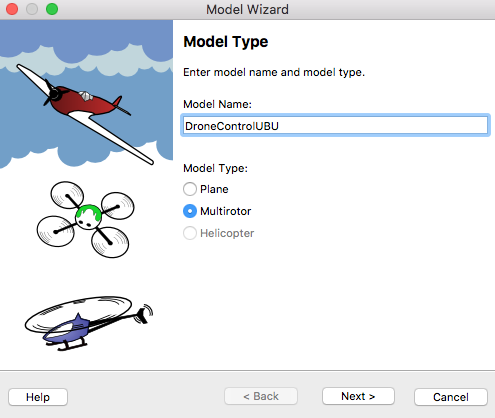
\includegraphics[width=0.7\textwidth]{opentxconfig1}
	\caption[Creación de modelos OpenTX. 1]{Creación de modelos mediante \emph{OpenTX}. Asistente de configuración}\label{fig:opentxconfig1}
\end{figure}

\item A continuación se muestra el orden de los canales. El sistema está preparado para interpretar el siguiente \emph{mapeo} de canales: 1-Acelerador (\emph{Throttle}), 2-Balanceo (\emph{Aileron}), 3-Elevación (\emph{Elevation}), 4-Rotación (\emph{Rudder}), 5-Armar/Desarmar (\emph{Arm/Disarm}).
En esta pantalla solo se muestran los cuatro primeros canales. El canal que permite armar o desarmar el drone se configurará más adelante.
\begin{figure}[H]
	\centering
	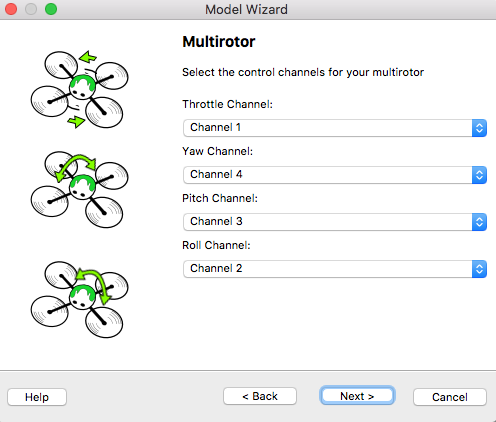
\includegraphics[width=0.7\textwidth]{opentxconfig2}
	\caption[Creación de modelos OpenTX. 2]{Creación de modelos mediante \emph{OpenTX}. Asistente de configuración}\label{fig:opentxconfig2}
\end{figure}
\item Se guardan los cambios realizados.
\begin{figure}[H]
	\centering
	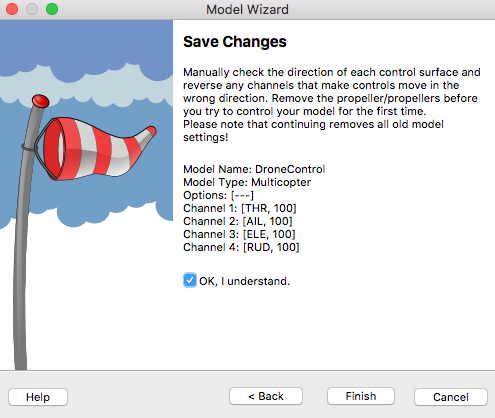
\includegraphics[width=0.7\textwidth]{opentxconfig3}
	\caption[Creación de modelos OpenTX. 3]{Creación de modelos mediante \emph{OpenTX}. Asistente de configuración}\label{fig:opentxconfig3}
\end{figure}
\item Y ya está casi listo el nuevo modelo. 
\item Se da doble click sobre él, para acceder a la configuración avanzada del mismo.
\begin{figure}[H]
	\centering
	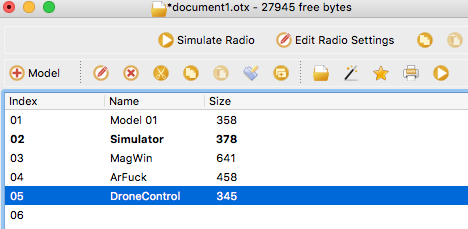
\includegraphics[width=0.7\textwidth]{opentxconfig4}
	\caption[Creación de modelos OpenTX. 4]{Creación de modelos mediante \emph{OpenTX}. Asistente de configuración}\label{fig:opentxconfig4}
\end{figure}
\item Desplazándonos hasta la parte inferior de la pestaña \emph{Setup}, se establece a <<OFF>> tanto \emph{Internal Radio System} como \emph{External Radio Module} (desactivando así las opciones de radio, ya que la usaremos como \emph{joystick}). Se establece el \emph{Trainer Port} a \emph{Slave/Jack} para que use el puerto USB como conexión para el \emph{joystick}.
\begin{figure}[H]
	\centering
	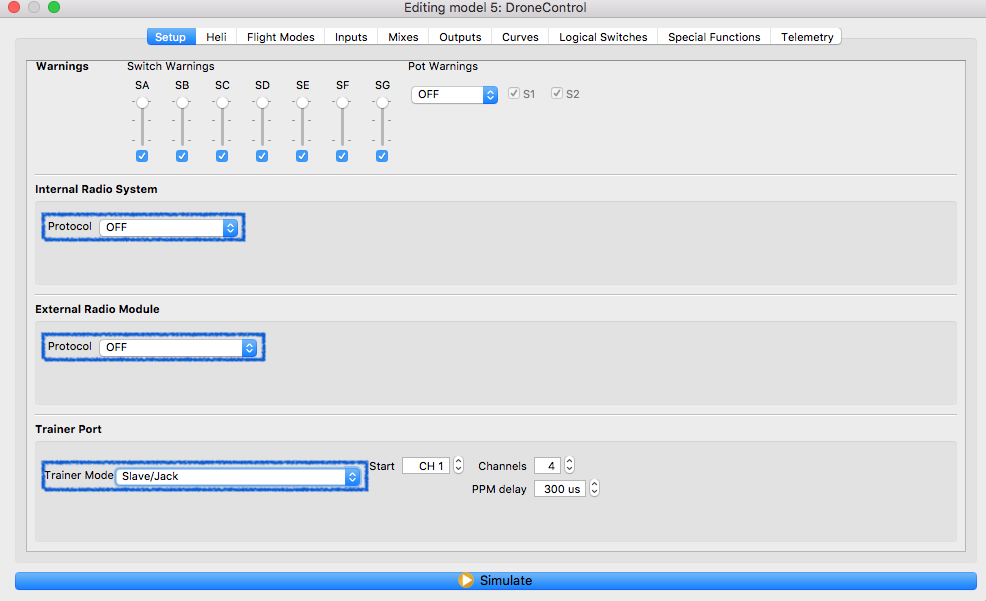
\includegraphics[width=0.7\textwidth]{opentxconfig5}
	\caption[Creación de modelos OpenTX. 5]{Creación de modelos mediante \emph{OpenTX}. Asistente de configuración}\label{fig:opentxconfig5}
\end{figure}
\item Se accede a la pestaña \emph{Inputs} (en ella se muestran los canales anteriormente configurados) y se añade uno nuevo dando doble click sobre el siguiente espacio vacío, correspondiente a \emph{I5}. 
\begin{figure}[H]
	\centering
	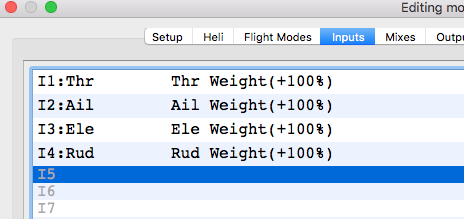
\includegraphics[width=0.7\textwidth]{opentxconfig6}
	\caption[Creación de modelos OpenTX. 6]{Creación de modelos mediante \emph{OpenTX}. Asistente de configuración}\label{fig:opentxconfig6}
\end{figure}
\item Se muestra ahora la configuración de un nuevo \emph{input}. Se le proporciona un nombre, \emph{Arm} en este caso, y se establece su \emph{Source} (fuente) a uno de los múltiples interruptores disponibles. En el caso de esta configuración, se ha establecido en el interruptor marcado como \emph{SF}, ya que es de fácil acceso.
\begin{figure}[H]
	\centering
	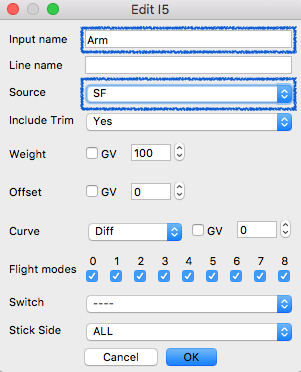
\includegraphics[width=0.5\textwidth]{opentxconfig7}
	\caption[Creación de modelos OpenTX. 7]{Creación de modelos mediante \emph{OpenTX}. Asistente de configuración}\label{fig:opentxconfig7}
\end{figure}
\begin{figure}[H]
	\centering
	\includegraphics[width=0.7\textwidth]{taranisSF}
	\caption[Interruptor SF de la emisora]{Interruptor SF de la emisora de fácil acceso.}\label{fig:taranisSFswitch}
\end{figure}

\item A continuación se asigna ese \emph{input} recién creado a un canal. Para ello se accede a la pestaña \emph{Mixes} y se selecciona el elemento \emph{CH5} de la lista.
\begin{figure}[H]
	\centering
	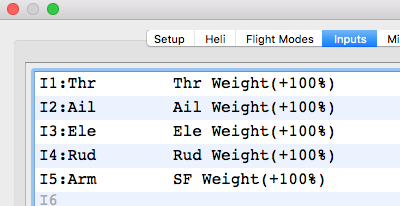
\includegraphics[width=0.7\textwidth]{opentxconfig8}
	\caption[Creación de modelos OpenTX. 8]{Creación de modelos mediante \emph{OpenTX}. Asistente de configuración}\label{fig:opentxconfig8}
\end{figure} 
\item Se da doble click sobre el elemento, y se configura el nombre y la fuente del canal, estableciendo esta al \emph{input} recién creado.
\begin{figure}[H]
	\centering
	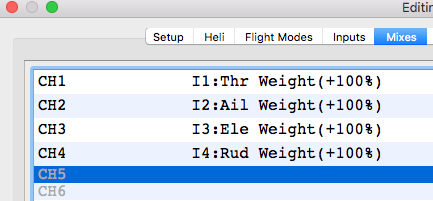
\includegraphics[width=0.7\textwidth]{opentxconfig9}
	\caption[Creación de modelos OpenTX. 9]{Creación de modelos mediante \emph{OpenTX}. Asistente de configuración}\label{fig:opentxconfig9}
\end{figure}
\item Con esto quedaría listo el modelo creado. 
\begin{figure}[H]
	\centering
	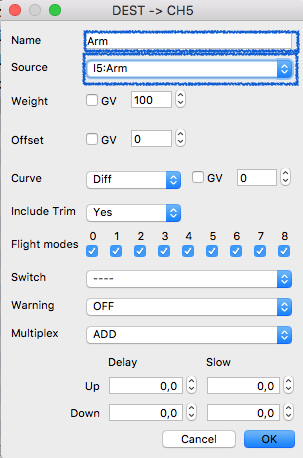
\includegraphics[width=0.5\textwidth]{opentxconfig10}
	\caption[Creación de modelos OpenTX. 10]{Creación de modelos mediante \emph{OpenTX}. Asistente de configuración}\label{fig:opentxconfig10}
\end{figure}
\item A continuación se escribe el modelo en la configuración de la emisora, pulsando sobre \emph{Write Models and Settings to Radio} y se pulsa sobre \emph{Write to TX} en la ventana emergente.
\begin{figure}[H]
	\centering
	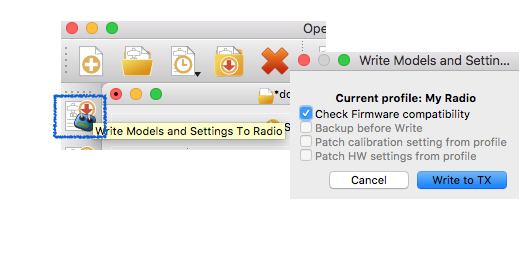
\includegraphics[width=0.7\textwidth]{opentxwrite}
	\caption[Escritura de modelos OpenTX.]{Escritura de modelos mediante \emph{OpenTX}.}\label{fig:opentxwrite}
\end{figure}
\end{enumerate}

Ahora la emisora dispone de un nuevo modelo, el cual se puede utilizar para manejar el drone a través de la interfaz web. Tan solo habría que seleccionarlo en el menú de la emisora, pulsando la tecla \emph{MENU}, desplazándonos hasta el modelo y presionando unos instantes la tecla \emph{ENT}. A continuación se selecciona \emph{Select model}.
\begin{figure}[H]
	\centering
	\includegraphics[width=0.8\textwidth]{taranismodels}
	\caption[Acceso a modelos de la emisora.]{Acceso a los diferentes modelos de la emisora.}\label{fig:taranismodels}
\end{figure}

\begin{figure}[H]
	\centering
	\includegraphics[width=0.7\textwidth]{taranisselectmodel}
	\caption[Acceso a modelo creado en la emisora.]{Acceso al modelo creado en la emisora.}\label{fig:taranisselectmodel}
\end{figure}

\begin{figure}[H]
	\centering
	\includegraphics[width=0.7\textwidth]{taranisDroneUBU}
	\caption[Uso de modelo creado en la emisora.]{Uso del modelo recién creado en la emisora.}\label{fig:taranisDroneUBU}
\end{figure}


\section{Manual del usuario}

Para utilizar la aplicación web, el usuario debe disponer de credenciales de acceso. Dichas credenciales solo pueden ser provistas por un administrador del servidor web. 

\subsection{Inicio de sesión}
\label{subsec:login}
Cuando disponga de ellas, el usuario puede dirigirse a la página creada a tal efecto, e iniciar sesión, tal y como se muestra en la Figura \ref{fig:userManualLogin}.


\begin{figure}[H]
	\centering
	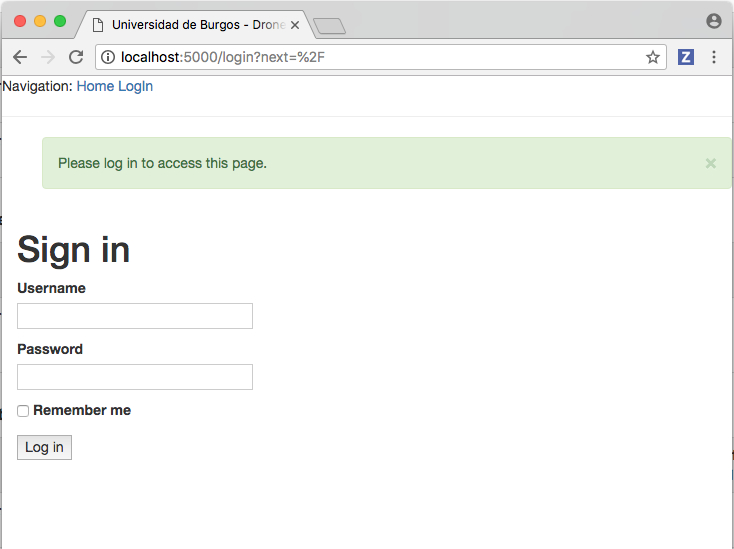
\includegraphics[width=0.7\textwidth]{userManualLogin}
	\caption[Inicio de sesión en la aplicación web.]{Inicio de sesión en la aplicación web.}\label{fig:userManualLogin}
\end{figure}

De intentar acceder al \emph{index} de la aplicación web directamente, sin haber realizado el inicio de sesión, redirigirá a la página de \emph{login}, mostrando un aviso informativo.

Si el usuario dispone de credenciales de acceso, y un \emph{drone} asignado, podrá acceder al sistema de control del dispositivo. Cabe destacar que las funcionalidades de sistemas automatizados se encuentran deshabilitadas, a falta de realizar más pruebas de campo.

\begin{figure}[H]
	\centering
	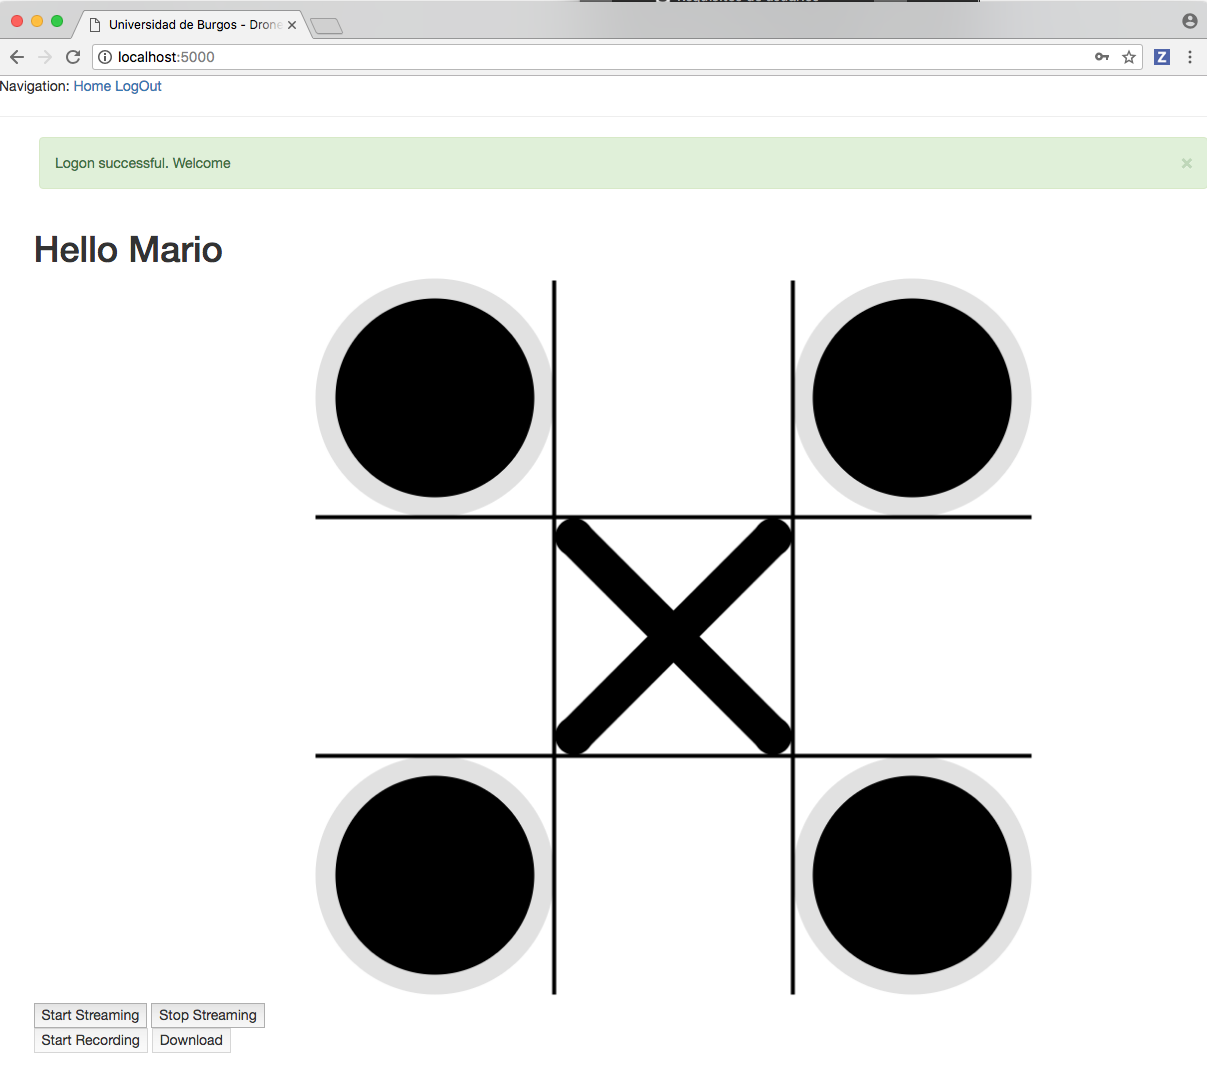
\includegraphics[width=0.8\textwidth]{userManualMainweb}
	\caption[Página principal de control del sistema.]{Página principal del sistema de control remoto del agente.}\label{fig:userManualMainweb}
\end{figure}


\subsection{Activación de vídeo}
\label{subsec:videoEnable}
El \emph{drone} dispone de una cámara que puede ser activada a demanda. Nada más iniciar sesión en la página, la aplicación web conecta con el \emph{drone} y le solicita que informe sobre la disponibilidad de vídeo bajo una configuración predefinida\footnote{Dicha configuración por el momento es fija, y se ha establecido en base a pruebas empíricas. Se hace uso de aceleración hardware para realizar el \emph{encoding} del vídeo a 1280$\times$720 a 15f/s. Será configurable en un futuro para llegar hasta una resolución de 1080p, aunque no se recomienda, dado el alto consumo de ancho de banda.}. De esta forma, en cuanto se solicita iniciar el vídeo, la aplicación ya dispone de la información necesaria para establecer la comunicación con el \emph{drone}.

Pulsando sobre el botón \emph{Start Streaming} se activa el vídeo disponible. Pulsando sobre el botón \emph{Stop Streaming} se detiene la emisión de vídeo. 

 
\begin{figure}[H]
	\centering
	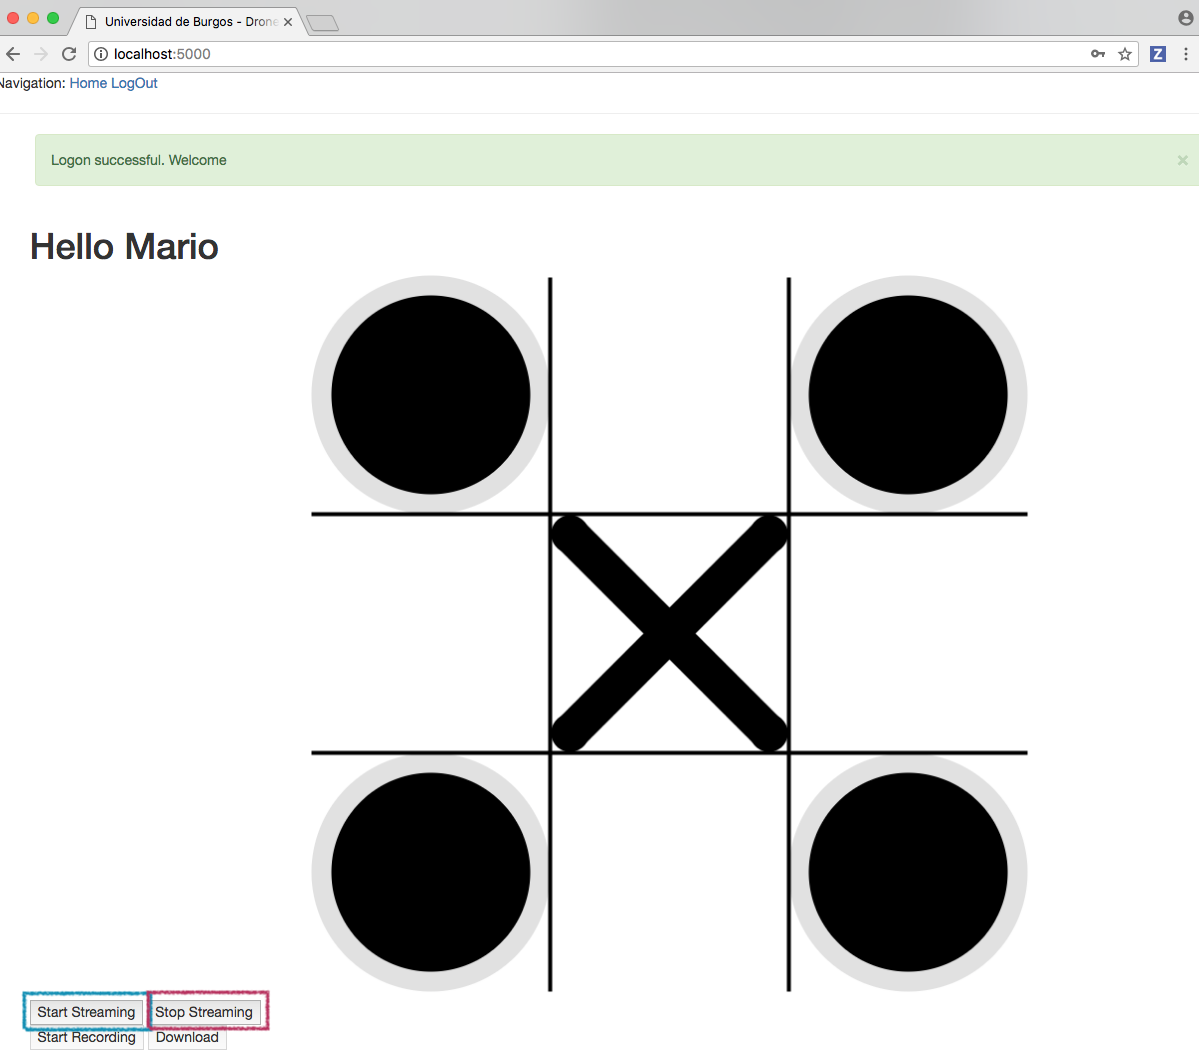
\includegraphics[width=0.9\textwidth]{userManualEnableVideo}
	\caption[Página principal. Gestión de vídeo.]{Página principal del sistema de control remoto del agente. Activación/Desactivación de vídeo.}\label{fig:userManualEnableVideo}
\end{figure}

\begin{figure}[H]
	\centering
	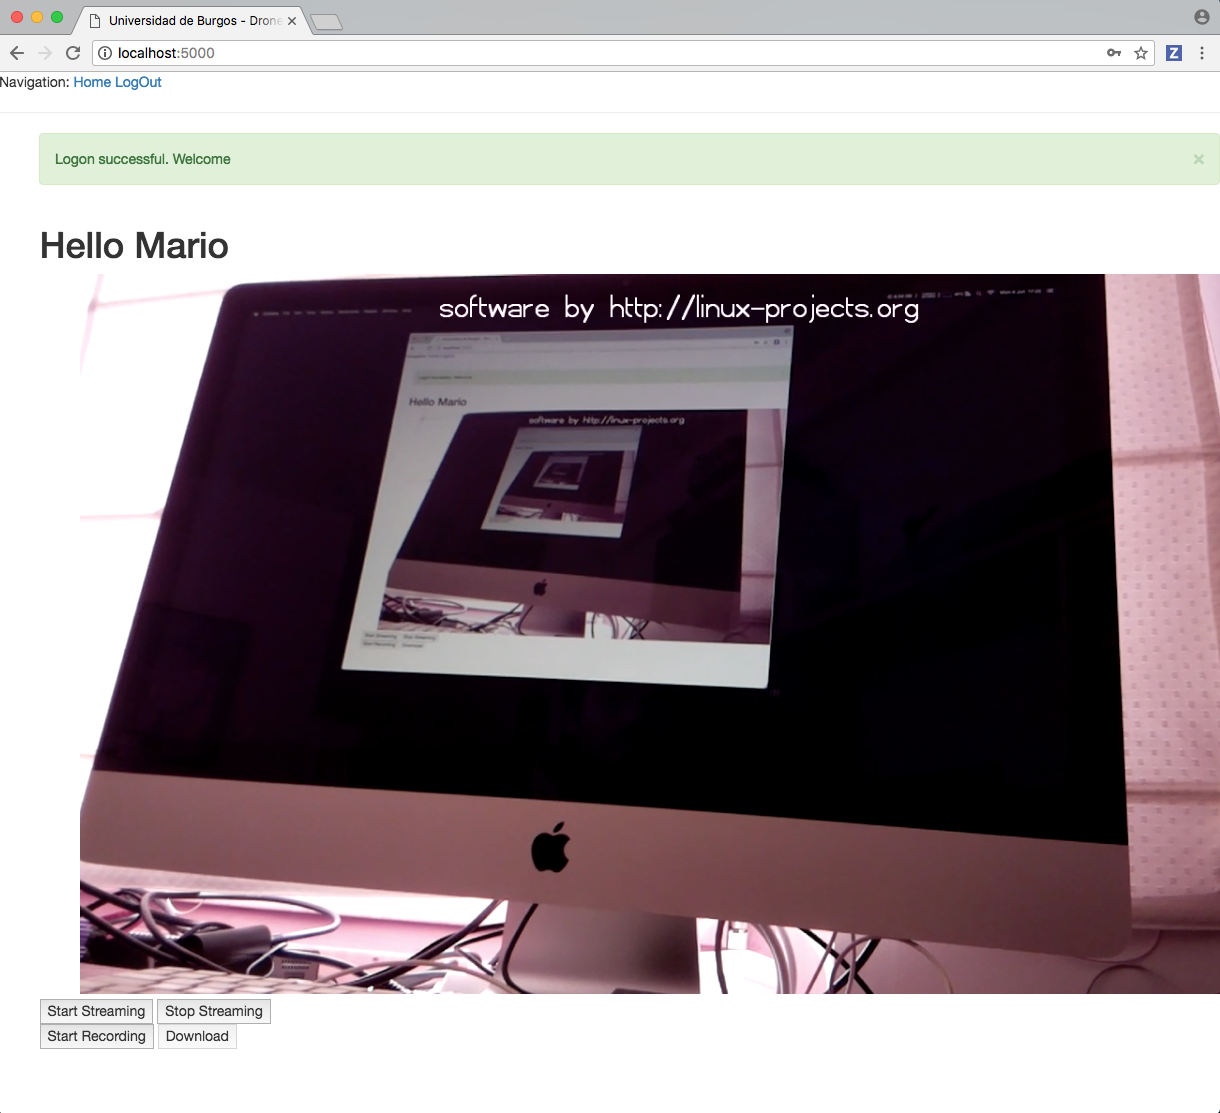
\includegraphics[width=0.9\textwidth]{samplevideo}
	\caption[Página principal. Gestión de vídeo.]{Página principal del sistema de control remoto del agente. Ejemplo de vídeo con luz diurna.}\label{fig:samplevideo}
\end{figure}

Cabe destacar que el color del vídeo no es perfecto. Esto es debido a la falta de un filtro de luz infrarroja en la cámara utilizada. Si bien durante el día el tono del color es <<rojizo>>, aporta la capacidad de disponer de visión nocturna haciendo uso de los LED infrarrojos instalados en el \emph{drone}. Dichos LED se activan automáticamente\footnote{Su funcionamiento está basado en un LDR, o \emph{Light Dependent Resistor}, o fotorresistor. Un componente cuya resistencia varía en función de la luz que detecta.} cuando las condiciones de luminosidad son bajas, y su luz no es visible al ojo humano. Sin embargo, la cámara del \emph{drone} es capaz de captarla. Los anillos de 36 LED infrarrojos aportan, en condiciones de baja luminosidad, una visibilidad perfecta a varios metros de distancia. 

\begin{figure}[H]
	\centering
	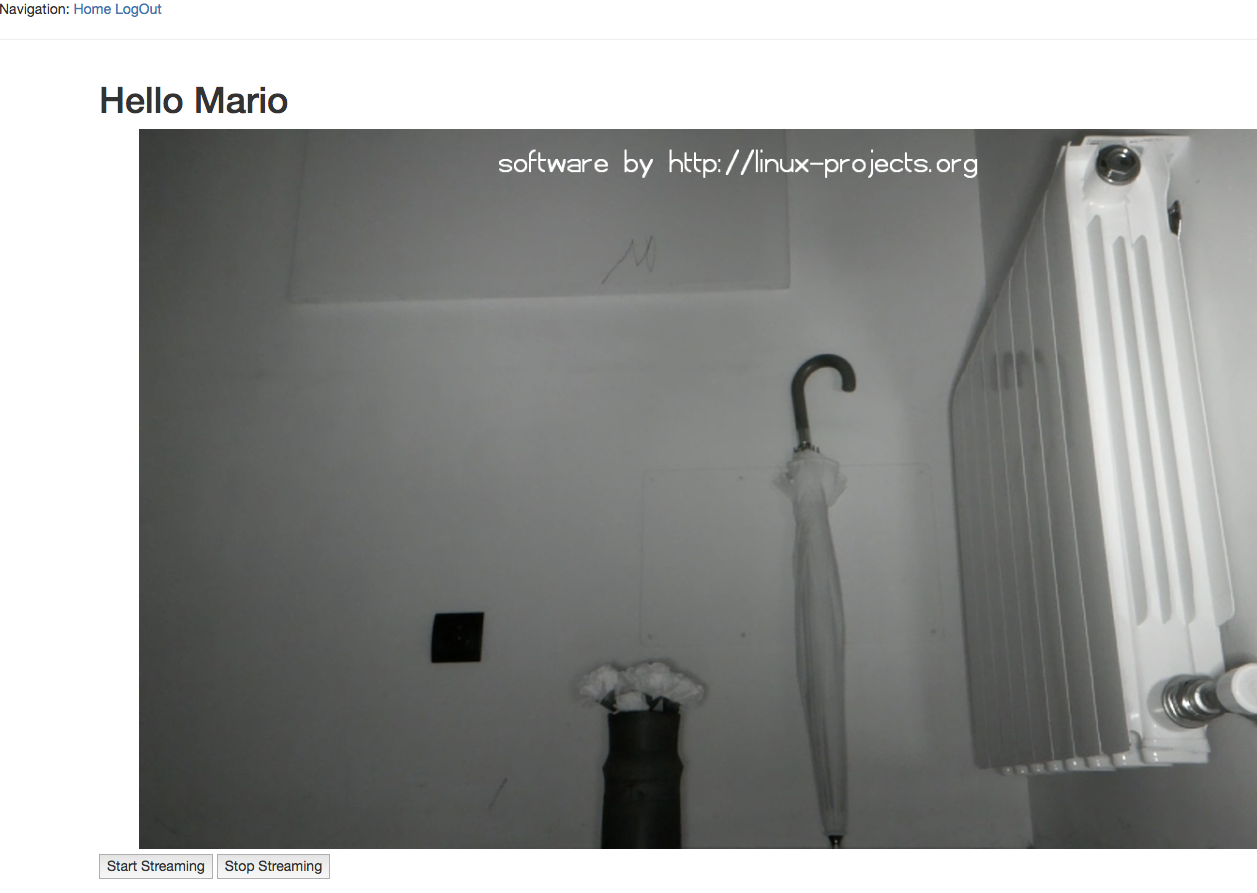
\includegraphics[width=0.9\textwidth]{vidStream}
	\caption[Página principal. Gestión de vídeo. Nocturno.]{Página principal del sistema de control remoto del agente. Ejemplo de vídeo con luz infrarroja.}\label{fig:samplevidenight}
\end{figure}


\subsection{Grabación de vídeo}
La interfaz web permite realizar grabación de vídeo. Basta con activar el vídeo, tal y como se explicó en la subsección \ref{subsec:videoEnable}, y pulsar sobre el botón \emph{Start Recording}. Cuando se desee detener la grabación se pulsará sobre el mismo botón, que habrá cambiado su nombre a \emph{Stop Recording}. Seguidamente el botón \emph{Download} se habrá activado. Bastará con pulsarlo para descargar un archivo \emph{.webm} con el vídeo grabado.

\begin{figure}[H]
	\centering
	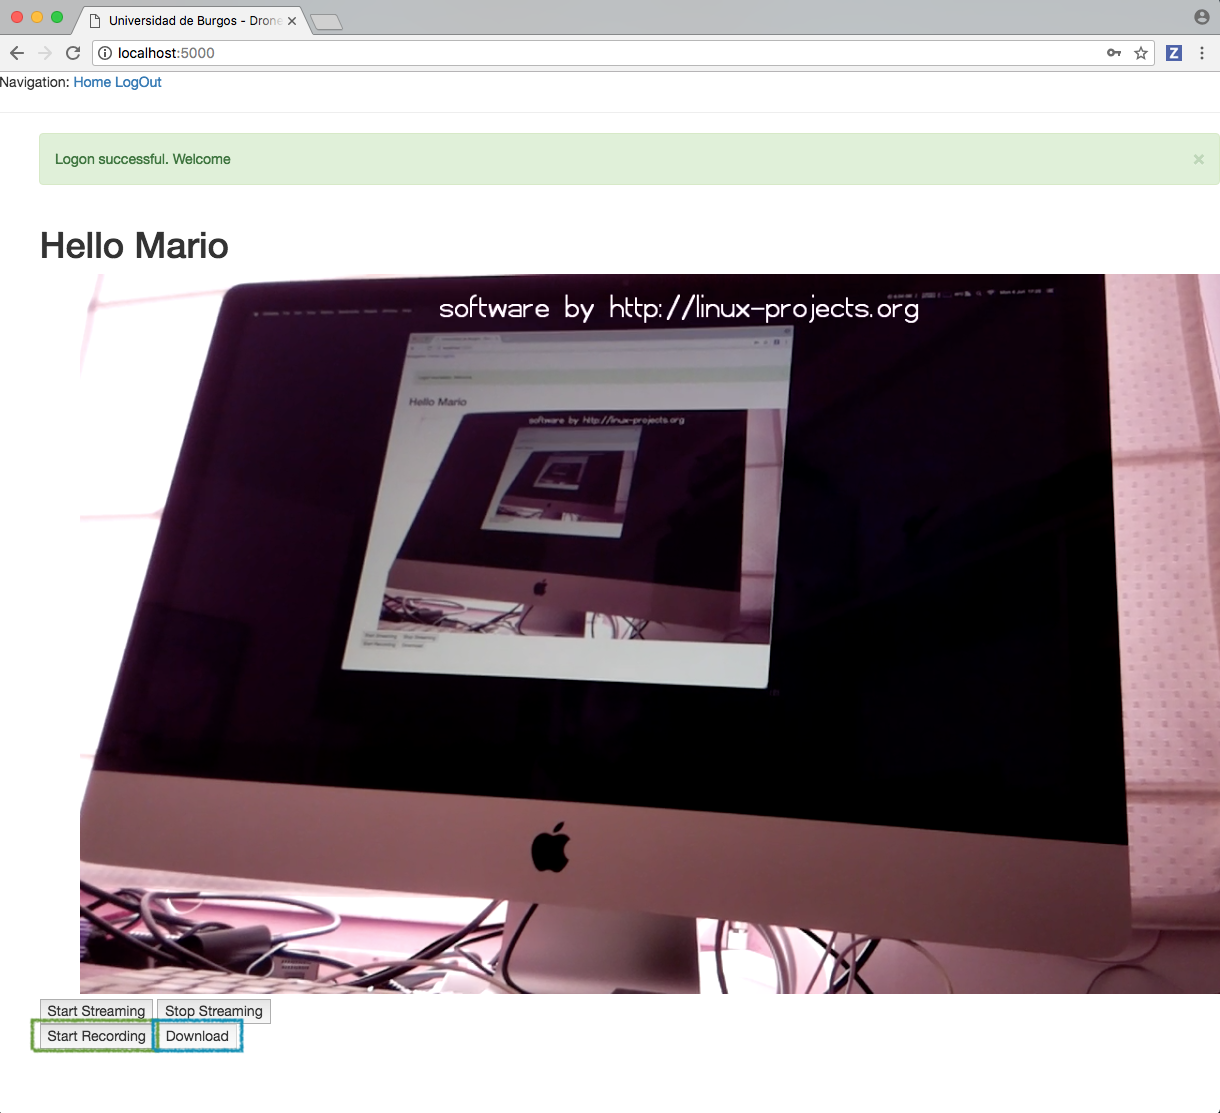
\includegraphics[width=0.9\textwidth]{videoRecording}
	\caption[Página principal. Gestión de vídeo. Grabación.]{Página principal del sistema de control remoto del agente. Grabación de vídeo.}\label{fig:userManualRecordVideo}
\end{figure}

\section{Modo manual}

Para activar el modo de control manual del \emph{drone} es necesario haber seguido los pasos para configurar la emisora, ver sección \ref{sec:instTaranis}. 

En primer lugar se deberá iniciar sesión en el sistema, tal y como se explicó en la sección \ref{subsec:login}. 
Una vez en la página de control del \emph{drone}, se conectará la emisora.

\noindent \textbf{NOTA IMPORTANTE}: Para que el sistema de control manual envíe la información de la emisora, y la reconozca, el navegador debe estar activo, es decir, no se deben realizar cambios de aplicación mientras el control manual esté activado, ya que se corre el riesgo de que este se desconecte. Esta restricción es parte de la API de JavaScript para el elemento \emph{Gamepad}, ver \href{https://developer.mozilla.org/en-US/docs/Web/API/Gamepad_API/Using_the_Gamepad_API}{Gamepad API} para más información.


Al conectar la emisora, está será reconocida de forma automática por la aplicación, y se permitirá activar el control manual mediante el botón \emph{Enable Manual}. 

\begin{figure}[H]
	\centering
	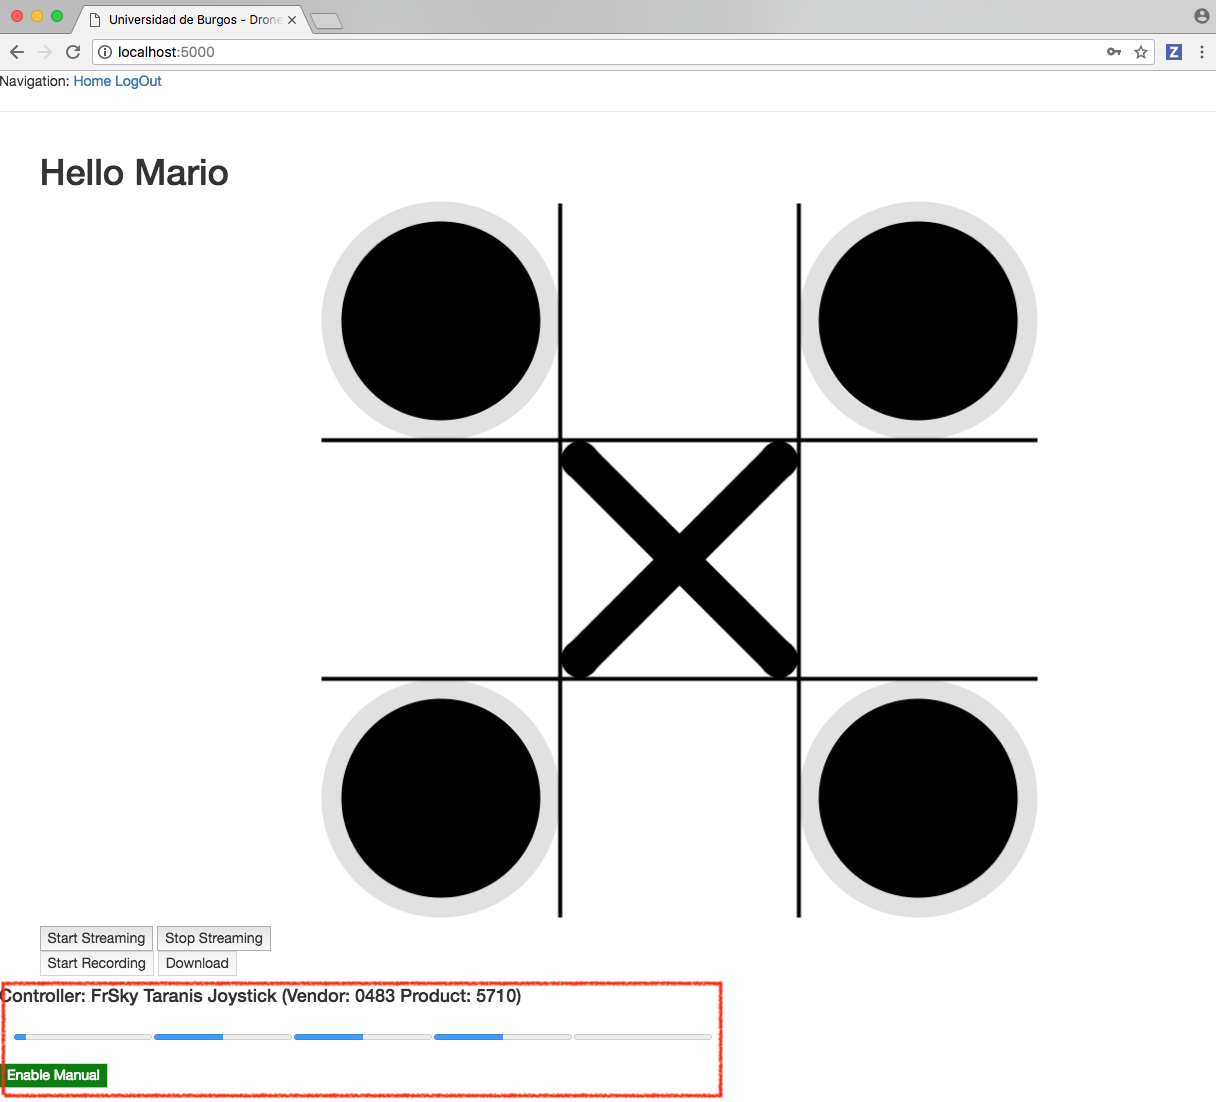
\includegraphics[width=0.9\textwidth]{manualMode}
	\caption[Página principal. Gestión de control manual.]{Página principal del sistema de control remoto del agente. Control manual del \emph{drone}.}\label{fig:manualMode}
\end{figure}

Como puede verse en la Figura \ref{fig:manualMode}, se ha reconocido la emisora, y se muestra el valor de los canales en forma de barra de progreso. 


Al activar el modo manual, el botón \emph{Enable Manual} cambiará su nombre a \emph{Disable Manual}, y su color a rojo. 

\begin{figure}[H]
	\centering
	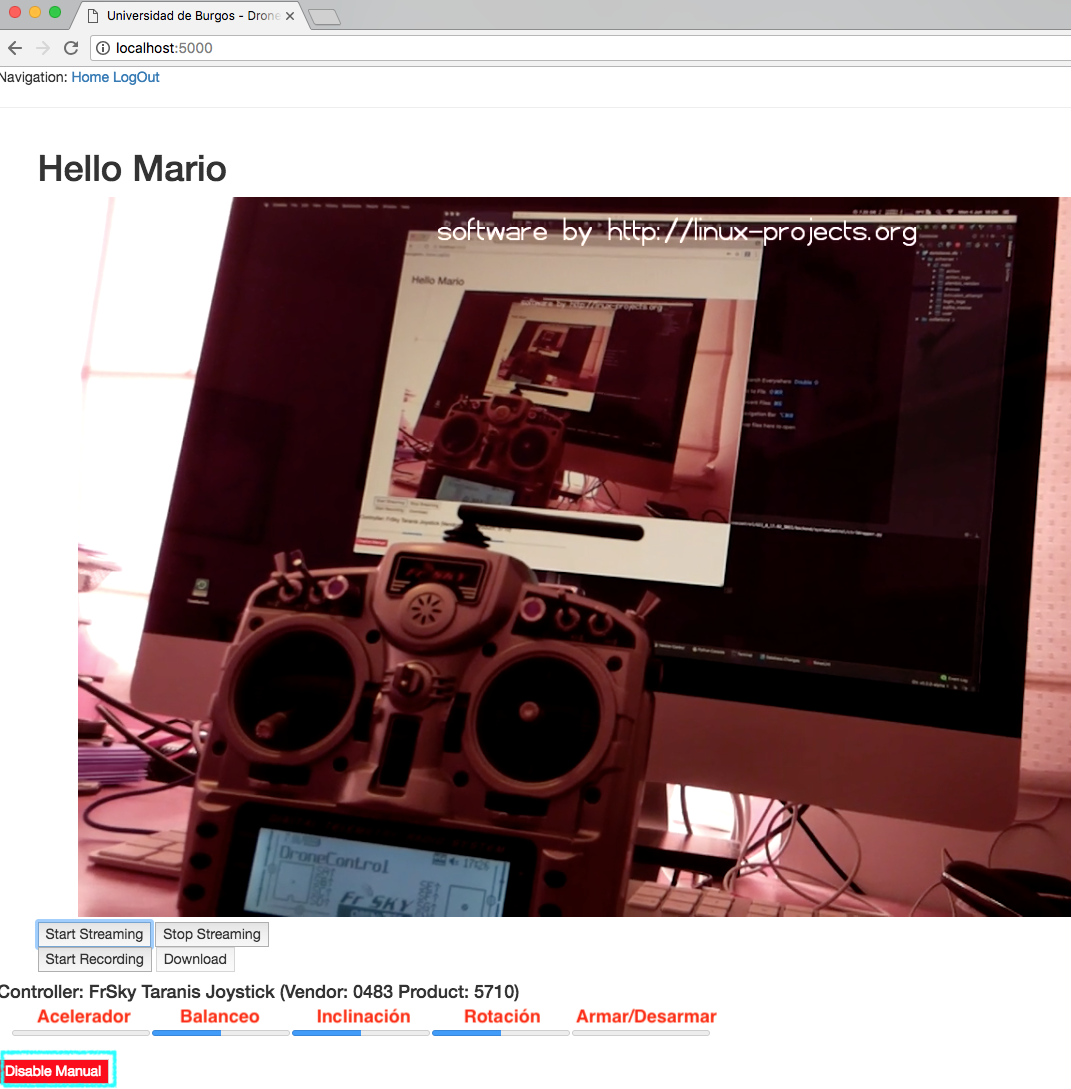
\includegraphics[width=0.9\textwidth]{droneReadytogo}
	\caption[Página principal. Gestión de control manual. Activación]{Página principal del sistema de control remoto del agente. Control manual del \emph{drone}. \emph{Drone} Activo.}\label{fig:droneReadytogo}
\end{figure}


\noindent \textbf{NOTA IMPORTANTE}: Desde este momento, el control del \emph{drone} se encuentra activo. NUNCA, bajo ninguna circunstancia, active el \emph{drone} cerca de personas o animales. Siempre deben observarse las medidas de seguridad detalladas en la subsección \ref{subsec:legislacion}. Este dispositivo no es, ni mucho menos, un juguete. Las hélices giran a una velocidad máxima de $13608$ rpm, y pueden causar daños o heridas graves, ver Figura \ref{fig:hand}. 

\begin{figure}[H]
	\centering
	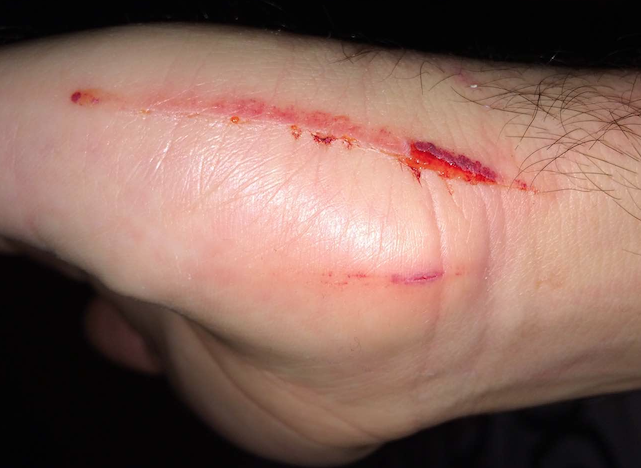
\includegraphics[width=0.7\textwidth]{hando}
	\caption[Herida producida por hélice del \emph{drone}]{Los experimentos, mejor con gaseosa.}\label{fig:hand}
\end{figure}


A continuación puede activarse, armarse, el \emph{drone} haciendo uso del interruptor que se designó en la sección \ref{sec:instTaranis}. 
Armar el \emph{drone} supone que las hélices comienzan a girar a velocidad baja. 

Se recomienda encarecidamente activar la emisión de vídeo si se va a operar el \emph{drone} de forma remota.






